\section{Results and analysis}

\begin{frame}<beamer>{Outline}
    \tableofcontents[currentsection,currentsubsection]
\end{frame}

\begin{frame}{Results - Time per Epoch}

		\begin{center}
		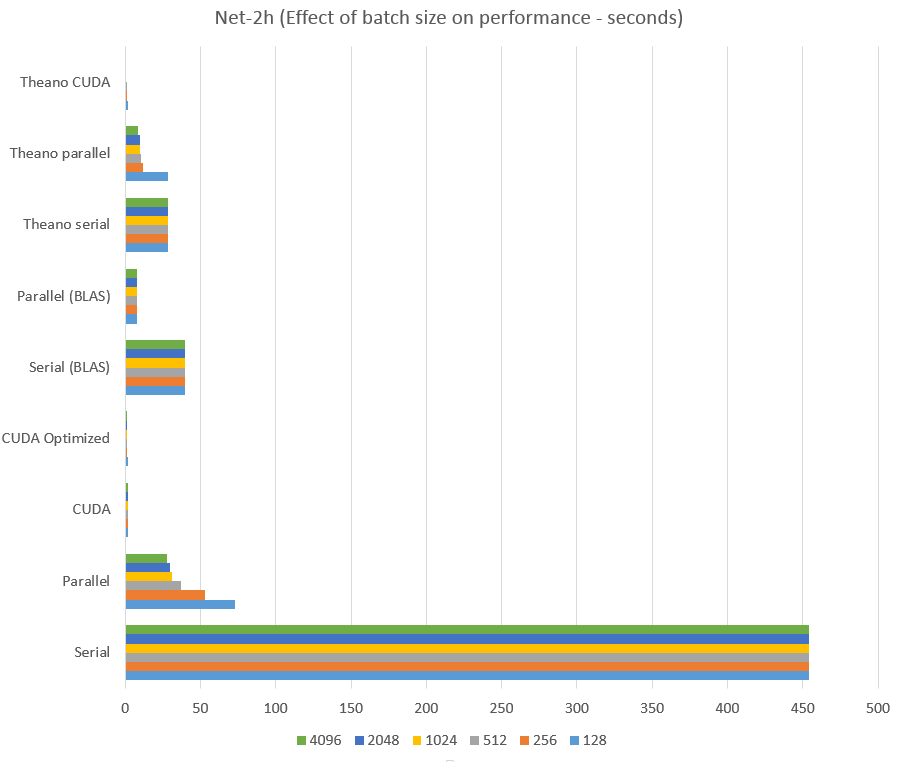
\includegraphics[width=0.7\textwidth]{net_2h_batch_secs.png}
		\end{center}

\end{frame}
 
\begin{frame}{Results - Gigaflops}
     
		\begin{center}
		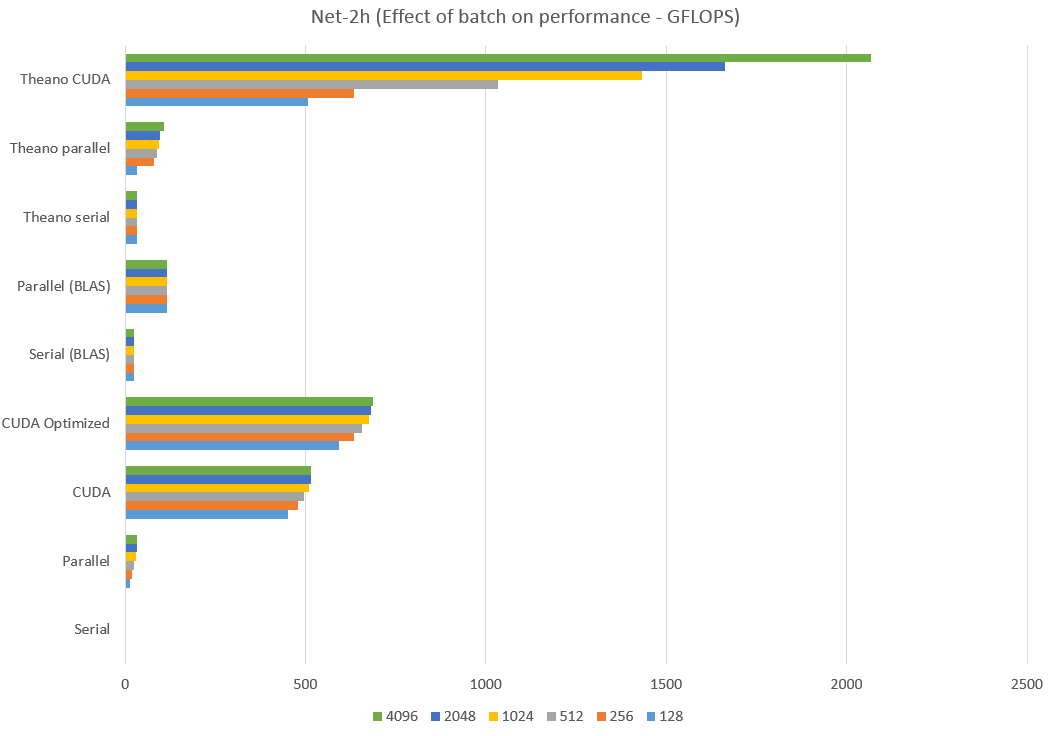
\includegraphics[width=0.85\textwidth]{net2h_batch_gflops.png}
		\end{center}

 \end{frame} 

\begin{frame}{Results - Speedup}
     
		\begin{center}
		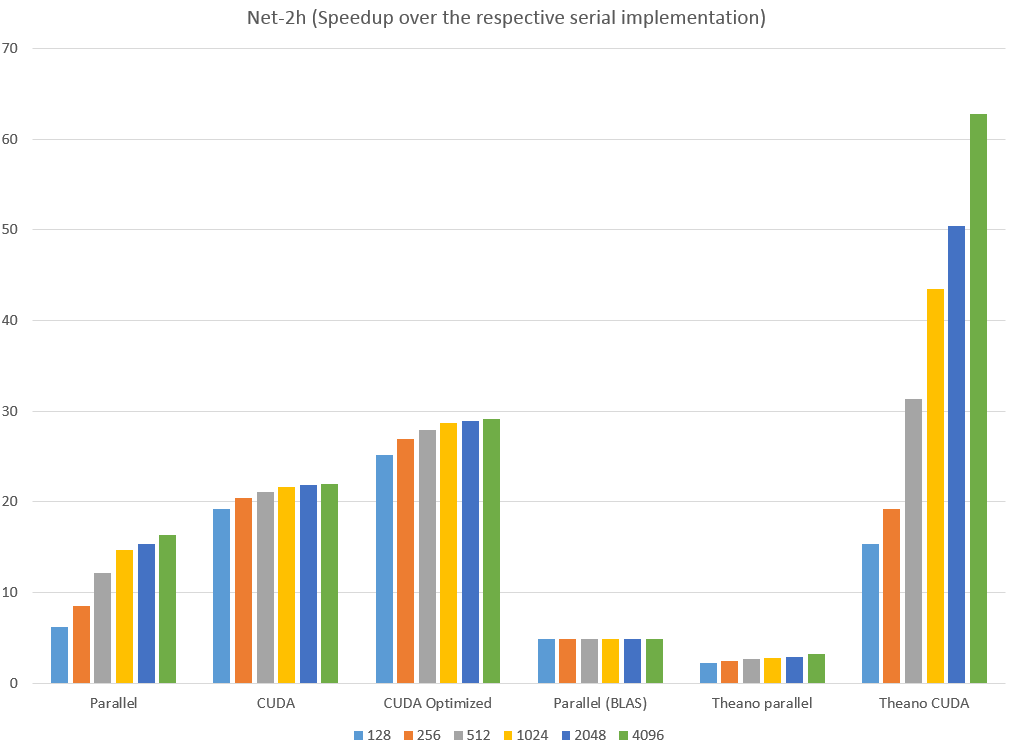
\includegraphics[width=0.8\textwidth]{net_2h_speedup.png}
		\end{center}

\end{frame}

 
\begin{frame}{Analysis}
 	\begin{itemize}
 	\item \textbf{Our implementation}
 	\begin{itemize}
 	\item Parallel computing average speedup $\approx 10$
 	\item Training time decreases as minibatch size decreases
 	\end{itemize}
 	\item \textbf{BLAS}
 	\begin{itemize}
 	\item Parallelizing each matrix vector product gives even faster results
 	\item Speedup independent of batch size, but less than our implementation
	\end{itemize}
	\item \textbf{CUDA}
	\begin{itemize}
	\item Our CUDA implementation gives about $\approx 20x$ speedup
	\item If \# neurons per layer are not perfect multiple of 32 then some threads do not participate in computation
	\end{itemize}
	\item \textbf{Theano}
	\begin{itemize}
	\item Apparently combines both types of parallelization
	\item Theano CUDA scales very fast with batch size
	\end{itemize}
 	\end{itemize}
 
\end{frame}
 
\begin{frame}{Future Work}

Combine the two parallelization techniques:
Split training examples amongst threads, further hierarchically parallelize matrix computations for each individual example.

\end{frame}

\begin{frame}{}

\begin{center}
Thank you \\
\vspace{25pt}
Questions?
\end{center}

\end{frame}



